\section{Applying RISE}
\nblink{nhs-chest-xray/analyze/rise.ipynb}
\nblink{nhs-chest-xray/analyze/rise\_bounding\_boxes.ipynb}

The implementation of RISE on the NIH Chest X-ray dataset with the DenseNet model was straightforward, because the reference implementation of RISE on GitHub \cite{risegithub} already
containes a working implementation for PyTorch. The implementation was not published on the Python Packaging Index, so the code had to be downloaded and added into our GitHub repository.

\subsection{Results}
\begin{figure}[H]
\centering
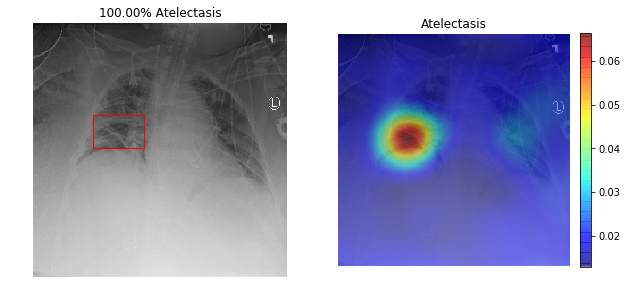
\includegraphics[width=12cm]{chapters/03_classification/images/rise_0.png}
\caption{The left image shows the input image with the bounding box added by a physician. The right image shows a RISE heat map and proofs that the neural network considers the correct part of the image as relevant for the correct classification}
\label{rise_example_1}
\end{figure}

\begin{figure}[H]
\centering
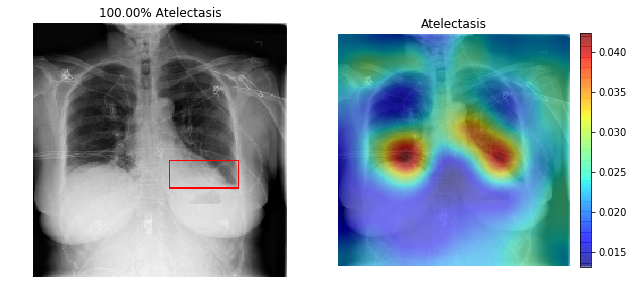
\includegraphics[width=12cm]{chapters/03_classification/images/rise_2.png}
\caption{The left image shows the input image with the bounding box added by a physician. The right image shows a RISE heat map and showing multiple regions that where important for the correct classification of this image.}
\label{rise_example_2}
\end{figure}

\begin{figure}[H]
\centering
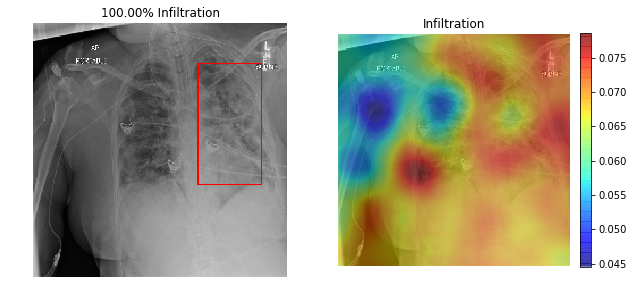
\includegraphics[width=12cm]{chapters/03_classification/images/rise_8.png}
\caption{The left image shows the input image with the bounding box added by a physician. The right image shows a RISE heat map where many regions which should be completely irrelevant for the classification are highlighted. The classification is still correct}
\label{rise_example_3}
\end{figure}

\subsection{Discussion}
Figure \ref{rise_example_1} shows that the bounding box created by a physician perfectly matches the region the neural network looked to came to the correct classification. In comparison, in Figure \ref{rise_example_2} the RISE heat map shows two regions which the neural network considers import for the correct classification. In this case, consultation with a physician is required if looking at those two places is correct for the diagnosis or if the neural network is wrong here.

As a last example, Figure \ref{rise_example_3} shows a heat map where regions are highlighted that should have no influence at all at a correct diagnosis. All three generated heat maps for this class (Infiltration) look similar, and are therefore an indicator that physicians can not depend on the correct diagnosis for this class.

Most heat maps look similar to the ones in Figure \ref{rise_example_2}, showing more regions relevant for the classification than the bounding boxes. This discrepancy has to be checked with a physician an is can not easily be dismissed as an error by the neural network.
